\documentclass[12pt]{article}
\usepackage[a4paper, bindingoffset=0.2in, %
							left=0.5in,right=0.5in,top=0.5in,bottom=0.5in,%
							footskip=.25in]{geometry}
\usepackage{graphicx}
\usepackage{amsmath}
\usepackage{physics}
\usepackage{hyperref}


\title{Midterm Report}
\author{Ali Abolhassanzadeh Mahani\\ 97110863}

\begin{document}
	\maketitle
	\section{Problem 1 (3D Site Percolation)}
	\subsection{Part a}
	I made a class \texttt{PercMatrix} that takes the length $L$ as the size of the arrays, and $p$, the probability with which I fill the cells with zero and on.
	Then, I go on and generate random binary numbers, and store shared poiters to them in the cells. I use smart pointers (\texttt{std::shared\_ptr<int>}) to make the clustering process faster.
	\subsection{Part b}
	First I make a $L\times L$ matrix called \texttt{frontier} that stores the color codes through out the clustering and coloring process. Then, I add a surface matrix called \texttt{init} to the beginning of the 
	cube that contains pointers to the cells in \texttt{frontier}. Then, I go through the cube cells and check if they are adjacent. If so, I form clusters, If more than one neighbors is on, I merge the cluster to the one with the lowest color code, since that cluster was made first.\\
	In the end, I check the ending surface of cube to see if any of the color code are between $1, L\times L +1$. If so, Percolation has occured. Otherwise, no percolation.
	In order to find the gyro radius, first, I find the color code of the biggest non-percolating cluster. Then, I 
	find the geometric center of that cluster and then, I can calculate the gyro radius.
	
	\section{Problem 2 (Erdos Renyi Graph)}
	\subsection{Part a (clustering)}
	I made the graph using \texttt{nx.erdos\_renyi\_graph(n, p)}. Here $p$ is the probablity of an edge to exist which is $\frac{<k>}{n}$ with $n$ being the number of nodes.\\
	I used the \texttt{nx.clustering(G)} module to calculate the clustering of each edge and then
	used a trick to store them in a \texttt{numpy array}. Then I plotted them using \texttt{plt.hist()}. (Fig\ref{fig:clust})
	\begin{figure}[h]
		\centering
		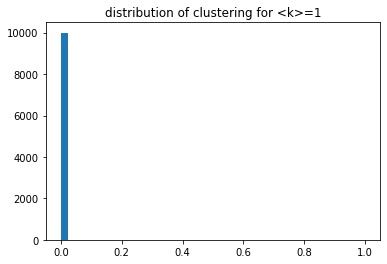
\includegraphics[width=.4\linewidth]{../p2/clust1.jpg}
		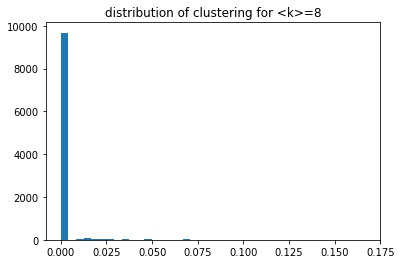
\includegraphics[width=.4\linewidth]{../p2/clust8.jpg}
		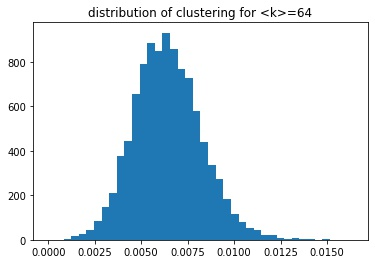
\includegraphics[width=.4\linewidth]{../p2/clust64.jpg}
		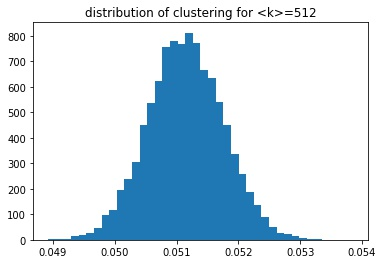
\includegraphics[width=.4\linewidth]{../p2/clust512.jpg}
		\label{fig:clust}
		\caption{clustering distribution for mean degrees of $\{1, 8, 64, 512\}$}
	\end{figure}
	\subsection{Part b (poisson dist. of degrees)}
	First I plot the histogram of degrees using \texttt{plt.hist()}, which gives me \texttt{counts}
	and \texttt{bins}, then I make a function that returns the probability using the poisson distribution. (basically made that function). Then, I found the poisson distribution of the \texttt{bins} and compared them to the actual \texttt{counts}. \\
	Then \texttt{np.sum} over them to find the cultivated error. The error is of order $\mathcal{O}(10^{-5})$ for $<k> = 64$
	
	This means that the poisson distribution function fits the degree distribution fairly well.
	\section{Problem 3 (Random Generation)}
	\subsection{Part a (generating function)}
	The function that generates this distribution is the inverse of $g(x)$. It is as follows:
	\begin{equation}
		g^{-1}(x) = \left(\frac{\alpha x_m^\alpha}{x}\right)^{\frac{1}{\alpha + 1}}
	\end{equation}
	In order to generate from $x_m$ to $\infty$, we need the input to be a uniform distribution
	from $0$ to $g^{-1}(x_m)$.\\
	I created this function and called it \texttt{target\_dist()}; then I made a random set of size 
	$100000$ and plotted the histogram as seen below.(Fig\ref{fig:reverse})
	\begin{figure}[h]
		\centering
		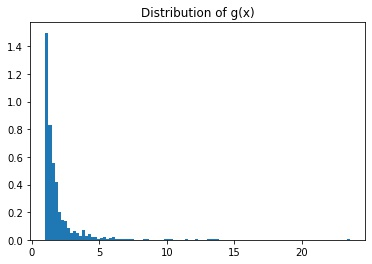
\includegraphics[width=.4\linewidth]{../p3/reverse.jpg}
		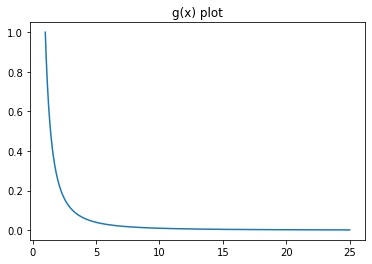
\includegraphics[width=.4\linewidth]{../p3/reverseplot.jpg}
		\label{fig:reverse}
		\caption{Distribution of $g(x)$ by 1000 samples and by ideal plot}
	\end{figure}
	
	\subsection{Part b (metropolis algorithm)}
	In the metropolis algorithm, first, I defined the function $g(x)$ to return it's value as states in the previous 
	subsection, and to return $0$ if $x \le 1$. Then, I made a function \texttt{gen\_dist(step, size)} which takes
	in the \texttt{step} and \texttt{size} and returns an array of random numbers as expected.
	Inside the function, I used two counters, one to count acceptances and one to count the whole process.
	Using the first, I can get the acceptance rate. I also stored all the numbers generated (whether or not they 
	were same)and using the second counter, I hand-picked the random samples.
	
	Then, I made a function \texttt{corr\_len()} that takes in all the numbers, calculates the auto correlation
	for values of $j = \{0, 10, 20, 30, \dots, 5000\}$. Then, I look to see at which point, the auto correlation becomes less than $e^{-1}$. That value of $j$ is our correlation (gyro) length.
	The results are in Table\ref{tab:gyro}
	\begin{table}[h]
		\centering
		\begin{tabular}{|c|c|c|c|c|c|c|c|c|c|}
			\hline
step size& $0.2$& $0.49$ & $0.9$ & $1.5$ & $2.45$ & $4$ & $6.4$ & $13.5$ & $33$ \\
 \hline
acceptance rate & $0.9$ & $0.8$ & $0.7$ & $0.6$ & $0.5$ & $0.4$ & $0.3$ & $0.2$ & $0.1$ \\
 \hline
correlation length & $5000$ & $1190$ & $3530$ & $430$ & $440$ & $290$ & $110$ & $1310$ & $90$ \\
 \hline
		\end{tabular}
	\label{tab:gyro}
	\caption{step size, and gyro length for different values of acceptance rate. The error for gyro length is 10.
	The first with gyro length 5000 suggests that the gyro is actually more for that acceptance rate since 5000
	is the maximum value in my calculations.}
	\end{table}

	\section{Problem 4 (simulation)}
	\textbf{List of group members:} \emph{Ali Abolhassanzadeh Mahani}, \emph{Abbas Shojakani}, \emph{Mohadeseh Asgari}
	\subsection{Stating the Problem}
	A blind /drunk person wants to cross a street using nothing but random process.\\
	We want to find his/her success rate relative to the degree of which how crowded the street is.\\
	We also want to find his/her mean lifetime for the times that he/she does not succeed and dies in a crash.
	\subsection{Simulation}
	The man is on the left side of the street at first, but then, It starts moving randomly with time.
	The boundary conditions are walls on the sides of the street. Meaning that if the man staeps to the left of the street, it stays there. If he reaches the right side, he succeeds.
	
	We took a mean of the car speeds and decided for it to be twice the speed of the blind/drunk person.
	The width of the street is fixed to size $L$ and the number of cars that are randomly generated and put on
	the street is our independent variable. The length of the cars is 1 unit area and the  
	cars move from bottom up. If in a time step, the position of the
	random walker and a car are interfered, the person is rendered dead, and is reset to be on the left side again. This cycle continues for the rest of the ensemble.\\
	We have also omitted the will of the drivers to hit the brake before hitting the person. So we have kind of assumed that the drivers are drunk too, which is a bit absurd or that the drivers' response time is not low enough to avoid a crash, which can be more reasonable.
	
	A better approximation of to set a condition to lower the speed if the driver sees the drunk person or that it
	shift the car to a new lane. Implementing these conditions can yield better, more accurate results. (We don't have time for that ;-) )
	\subsection{The Simulation Code}
	I made a random walker in 1 Dimension that randomly crosses the street. And every time it makes a choice, its lifetime is incremented by 1 unit time. This method \texttt{next()} that contains the decision making,
	returns 0 if the person is still in the street and returns 1 if the person has reached the right side (success).\\
	\emph{Mohadeseh} made the street and the cars that are randomly generated at the bottom of the street and move upwards with speed 40 unit length.\\
	\emph{Abbas} simulated using our code and got the statistics. The conditions of death and taking the mean are of his work. The precedence of time step evolution is with the random walker. Meaning first, the
	random walker takes a step, then the cars move with their speed. If the cars hit the man in their evolution
	process, the man dies, else, the loop continues until either the man reaches the other side of the street,
	or he dies in a crash.\\
	I also added a some code to get the mean life span for the times that the drunk person dies.
	Afterwards, I spent time refining the code, commenting it and making it pretty :)
	The results are below.
	
	In our work, the evolution of the cars up the street is a cellular automata and the person crossing the
	street is obviously a random walk simulation.
	\subsection{Results}
	 We simulated for the car speed $v = 40$ and the man's speed $V_p = 2$ and the street width $L = 10$.
	 Then, we plotted the success rate vs. the number of cars and the mean life span vs. the number of cars.
	 Fig\ref{fig:drunk}
	 \begin{figure}[h]
	 	\centering
		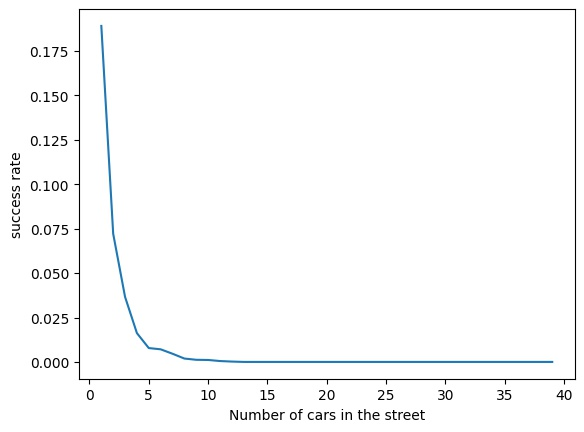
\includegraphics[width=.4\linewidth]{../p4/success.jpg}
		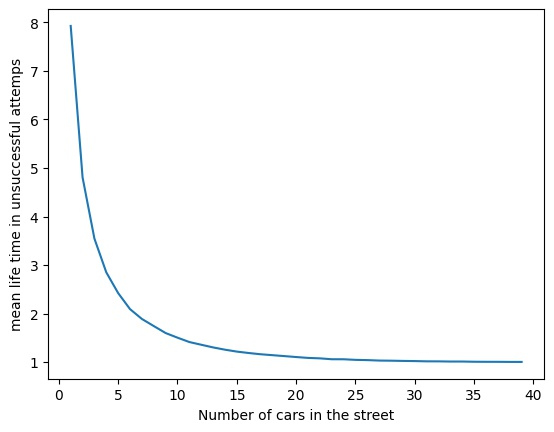
\includegraphics[width=.4\linewidth]{../p4/meanlife.jpg}
		\label{fig:drunk}
		\caption{On the left we have the success rate vs. the number of cars, and on the right we have
		the mean life time vs. the number of cars}
	 \end{figure}
 	As one can observe, the \emph{success rate} decays fast with \emph{number of cars}, the mean life time
 	also decays fast but a bit smoother than the success rate. The moral lesson here is that one shall not try crossing a street while drunk.
 	
 	The results show that for example, for a mean degree of crowd about 1 car per 100 unit area, the success rate is about $0.20$ and the mean lifetime for the unsuccessful times, it roughly 8 time steps.
 	for 10 cars per 100 unit area, those numbers decay to about $0$ and $1.5$ respectively.
 	In the ladder case, the drunk person dies after taking about $1.5$ steps in the street.\\
 	This threshold of $10$ can be due to the fact that the width of our street is 10 and since the \texttt{death\_check}'s conditions are perdiodic, for a velocity of 40 unit length per unit time, the entire street becomes full and the drunk person gets hit in just 1 or steps.
\end{document}
